%=================================================
% Economics Coursework Template
%=================================================
\documentclass[12pt]{article}

%------------ Packages ------------
\usepackage[margin=1in]{geometry}   % Page layout
\usepackage{lmodern}                % Latin Modern (LaTeX default font)
\usepackage{amsmath, amssymb}       % Math symbols
\usepackage{booktabs}               % Professional tables
\usepackage{graphicx}               % Figures
\usepackage{natbib}                 % References
\usepackage[hidelinks]{hyperref}    % Hyperlinks
\usepackage{fancyhdr}               % Headers/footers
\usepackage{setspace}               % Line spacing
\usepackage{titlesec}               % Section formatting
\usepackage{comment} 
\usepackage{xcolor} 
\usepackage{amsthm} 
\usepackage{float} 
\usepackage{dcolumn}
\usepackage{titlesec}
\usepackage{enumitem}
\usepackage{hyperref}
\usepackage{tikz}
\usepackage{multicol}
\usetikzlibrary{arrows.meta,positioning,fit,calc}
\tikzset{
  var/.style={rectangle, draw, rounded corners, minimum width=18mm, minimum height=7mm, align=center},
  latent/.style={ellipse, draw, dashed, minimum width=18mm, minimum height=7mm, align=center},
  controlarrow/.style={->, dashed, draw=red!60},
  lightbluearrow/.style={->, dashed, draw=blue!40} % NEW style
}

%------------ Page Style ------------
\rhead{\thepage}
\lhead{ECO1465 Weekly Report 1}

%------------ Section Formatting ------------
\titleformat{\section}{\large\bfseries}{\thesection.}{0.5em}{}
\titleformat{\subsection}{\normalsize\bfseries\itshape}{\thesubsection}{0.5em}{}
\titlespacing*{\subsection}{0pt}{1.5ex plus 1ex minus .2ex}{1em} % spacing before/after subsections


%------------ Begin Document ------------
\begin{document}
% Title Page only
\begin{titlepage}
    \thispagestyle{empty} % no headers/footers
    \centering
    \vspace*{\fill}

    {\Large \textbf{Linear Demand–Supply Model} \par}

    \vspace{3em}
    {\large Nardeen Abdulkareem \par}
    {\normalsize The University of Toronto \par}
    {\normalsize \today \par}
    {\texttt{nardeen.abdulkareem@mail.utoronto.ca} \par}

    \vspace*{\fill}
\end{titlepage}
\clearpage

\section{Equilibrium}
$$Q_D = \alpha_0 + \alpha_1P + \alpha_2Y + \mu_D$$
$$Q_S = \beta_0 + \beta_1P + \beta_2W + \mu_S$$
$$Q_D = Q_S = Q^*$$
$$\alpha_0 + \alpha_1P + \alpha_2Y + \mu_D = \beta_0 + \beta_1P + \beta_2W + \mu_S$$
$$P^* = \frac{\beta_0 + \beta_2W + \mu_S - \alpha_0 - \alpha_2Y - \mu_D}{\alpha_1 - \beta_1}$$
$$Q(P^*) = Q^* = \alpha_0 + \alpha_1(\frac{\beta_0 + \beta_2W + \mu_S - \alpha_0 - \alpha_2Y - \mu_D}{\alpha_1 - \beta_1}) + \alpha_2Y + \mu_D$$

Our parameters $(\alpha_i, \beta_i)$ yield the marginal effect of the increase in their associated variables. $(\alpha_1, \beta_1)$ inform us about the slope of our demand and supply curves with respect to prices. In the subsequent parts of this problem set we are informed that we have a downward negative sloping demand and an upward positive sloping supply curve which yields a denominator of ($\beta_1 - \alpha_1$). The larger the difference in magnitude in the denominator the less susceptible our price is to observed and unobserved shocks in our simple linear set up. Since quantity is a function of prices and shocks, when the price are less susceptible to shocks, due to a larger difference in magnitude of the price functions denominator, we can observe a dampened effect on quantities produced when a shock to the shifters occurs. Moving on, ($\alpha_0, \beta_0$) governs the intercepts for our supply and demand equations. Assuming that our unobserved demand and supply shocks ($\mu_S, \mu_D$) are defined as mean zero and independent across markets. We can state that the intercept terms decides how the supply and demand lines will shift due to uniform shifts across all consumers or suppliers. ($\mu_S, \mu_D$) are essentially the source of variation in our model, it allows for mean zero (homoskedastic?) residuals in our model. The difference between the intercept terms ($\alpha_0, \beta_0$) and the error terms ($\mu_S, \mu_D$) is how persistent baseline determinants of supply and demand that are captures in the intercepts. The intercept informs us about the choke price and the entry cost and the error term gives us the variation at each price and quantity. ($\alpha_2, \beta_2$) inform us about how prices and the subsequent quantities will shift due to a shock in observed supply and demand. These shocks on the demand side may include demographics, expectations, and revealed preferences. While supply side shocks are can be related to technology, and the marginal cost to producing a good. A demand shock will yield an increase in both quantity and price. I also believe that equilibrium price will rise more than equilibrium quantity since a price increase influences quantities negatively. On the supply side, a shock will cause the price to fall and quantity to rise. The equilibrium quantity will rise more than the price will decrease since a price fall enters the quantity function endogenously.
\newpage
\section{OLS and 2SLS}
\begin{table}[!htbp] \centering 
  \caption{Regression Table} 
  \label{} 
\small 
\begin{tabular}{@{\extracolsep{5pt}}lcccc} 
\\[-1.8ex]\hline 
\hline \\[-1.8ex] 
\\[-1.8ex] 
& \multicolumn{2}{c}{\textit{OLS}} 
& \multicolumn{2}{c}{\textit{IV}} \\ 
\cline{2-5} \\[-1ex]
& \textit{Demand} & \textit{Supply} 
& \textit{Demand} & \textit{Supply} \\ 
\hline \\[-1.8ex]
 Price & $-$0.42$^{***}$ (0.08) & 0.74$^{***}$ (0.08) & $-$2.14$^{***}$ (0.16) & 2.97$^{***}$ (0.33) \\ 
  Demand Shock & 0.71$^{***}$ (0.05) &  & 0.98$^{***}$ (0.07) &  \\ 
  Supply Shock &  & 1.15$^{***}$ (0.06) &  & 1.98$^{***}$ (0.14) \\ 
  Intercept & 22.46$^{***}$ (0.66) & 20.79$^{***}$ (0.58) & 31.07$^{***}$ (1.04) & 5.18$^{**}$ (2.29) \\ 
 \hline \\[-1.8ex] 
Observations & 1,000 & 1,000 & 1,000 & 1,000 \\ 
R$^{2}$ & 0.15 & 0.30 & $-$0.26 & $-$0.22 \\ 
Adjusted R$^{2}$ & 0.15 & 0.30 & $-$0.26 & $-$0.22 \\ 
Residual Std. Error (df = 997) & 0.82 & 0.75 & 1.01 & 0.99 \\ 
F Statistic (df = 2; 997) & 89.63$^{***}$ & 213.84$^{***}$ &  &  \\ 
\hline 
\hline \\[-1.8ex] 
\textit{Note:}  & \multicolumn{4}{r}{$^{*}$p$<$0.1; $^{**}$p$<$0.05; $^{***}$p$<$0.01} \\ 
\end{tabular} 
\end{table} 

(3c) Since there are no unobserved demand and supply shocks entering into the OLS regression above, we can observe that we have an endogenous price entering into the equation. Where the unobserved demand (supply) shock is correlated with price. This aforementioned case is that of omitted variable bias, but another explanation may be simultaneous causality bias. Simultaneous causality bias can explain how unobserved supply (demand) shocks enter the demand (supply) regression. When the unobserved supply shock enters the demand equation through the price, it shifts both the price and the quantities, allowing for price and quantities to move simultaneously.

(4a) We chose the observed demand (supply) shock as the instrument for price in the supply (demand) equation. The first justification for these instruments is that the demand (supply) shock is correlated with the prices since it enters into the equilibrium price equation from (1); this satisfies the relevance restriction of IV. The second justification for these instruments is that they only influence the quantities demanded (supplied) through the price. This means that since ($\mu_S, \mu_D$) are assumed to be independent across markets. ($W,Y$) only enter the demand and supply equations through price and are uncorrelated with the unobserved demand or supply shocks. 

(4c) The 2SLS results are very close to the parameters we have used to generate our data. This indicates that our conclusions from part 4a are correct and there exists some bias when we leave the unobserved supply and demand shocks out of the equation. We can say in this case, the implementation of 2SLS was sufficient to control for the variation in equilibrium prices that is driven by a mixture of unobserved demand and supply shocks. The 2SLS now generates exogenous variation in price.
\newpage
\section{Counter-factual Simulations}
An introduction of a per-unit tax introduces the issue of tax incidence. The problems becomes framed regarding who pays the tax, the producers or the consumer?
$$P_f = P_c - t$$
\text{Where} $P_f$ \text{is the price received by the firm and} $P_c$ \text{is the price paid by the consumer}
$$Q_D = \alpha_0 + \alpha_1P_c + \alpha_2Y + \mu_D$$
$$Q_S = \beta_0 + \beta_1(P_c - t) + \beta_2W + \mu_S$$
$$Q_D = Q_S = Q^*$$
$$\alpha_0 + \alpha_1P_c + \alpha_2Y + \mu_D = \beta_0 + \beta_1(P_c - t) + \beta_2W + \mu_S$$
$$P_c^* = \frac{\beta_0 + \beta_2W + \mu_S - \alpha_0 - \alpha_2Y - \mu_D - \beta_1t}{\alpha_1 - \beta_1}$$
$$Q(P_c^*) = Q^* = \alpha_0 + \alpha_1(\frac{\beta_0 + \beta_2W + \mu_S - \alpha_0 - \alpha_2Y - \mu_D - \beta_1t}{\alpha_1 - \beta_1}) + \alpha_2Y + \mu_D$$
$$P_f^* = P_c^* - t$$
In this case, we can expect the consumer price rise with an increase in taxes since: $$\frac{\partial P_c^*}{\partial t} = \frac{-\beta_1}{\alpha_1 - \beta_1} > 0$$ And, we can expect that the price producers receive for the good falls with an increase in the tax since: $$\frac{\partial P_f^*}{\partial t} = \frac{\partial P_c^*}{\partial t} - 1 = \frac{-\alpha_1}{\alpha_1 - \beta_1} < 0$$
The following are taken from Jean Tirole's, \textit{The Theory of Industrial Organization}, Introduction:
$$\text{Consumer Surplus (CS)} = \int_{P_c^*}^{P_{max}}Q_d(P)dP = \frac{1}{2}Q^*(P_{max} - P_c^*)$$
$$\text{Change in Consumer Surplus } (\Delta CS) = \int_{P_0}^{P_1}Q_d(P)dP$$
$$\text{Producer Surplus (PS)} = \int_{P_{min}}^{P_f^*}Q_s(P)dP = \frac{1}{2}Q^*(P_{f}^* - P_{min})$$
$$\text{Tax Revenue } = t \times Q^*$$
$$\text{Dead-Weight Loss (DWL) } \approx \frac{1}{2}t(Q_1 - Q^*)$$ Where $Q_1$ refers to the equilibrium quantities before the unit tax was imposed. These equations suggest that taxation will increase the dead weight loss by an amount that is smaller than the tax revenue generated by the government. A unit tax will cause inefficiencies in the market, which cases the total surplus (CS + PS) to fall. The extent that the producer and consumer surplus falls by is determined by the slope of the supply and demand equations. 
\newpage
\section{Empirical Impact}
The plot interpretations reflect what we previously discussed. CS and PS are decreasing with an increase in tax. TR is increasing and dimishing with an increase in tax. And DWL is increasing and convex with an increase in tax.

\begin{figure}[h]
\centering
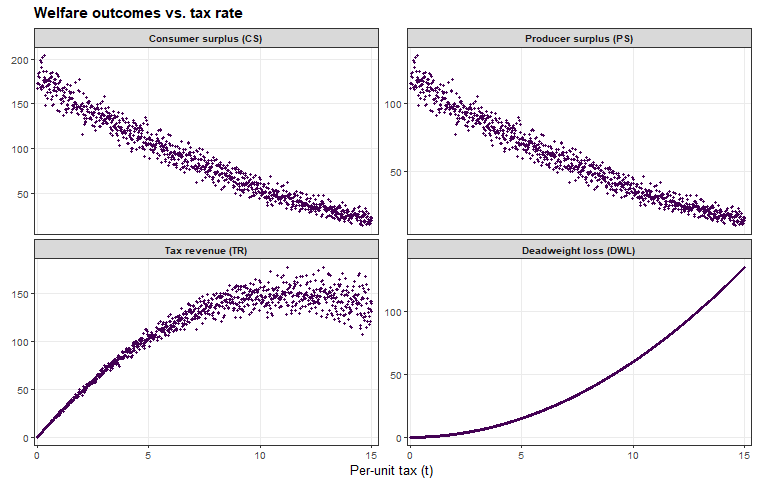
\includegraphics[width=\linewidth]{1.png}
\end{figure}


























\end{document}